\documentclass[12pt,addpoints]{exam}
\usepackage{enumitem}
\usepackage{amsfonts,amssymb,amsmath, amsthm}
\usepackage{graphicx}
\usepackage{systeme}
\usepackage{pgf,tikz,pgfplots}
\pgfplotsset{compat=1.15}
\usepgfplotslibrary{fillbetween}
\usepackage{mathrsfs}
\usetikzlibrary{arrows}
\usetikzlibrary{calc}
\pagestyle{headandfoot}
\firstpageheadrule
\runningheader{Grade 10 Workbook Problems}{}{Page \thepage\ of \numpages}
\runningheadrule
\author{St John Baptist De La Salle Catholic School, Addis Ababa}
\usepackage{geometry}
\firstpagefooter{}{}{}
\runningfooter{}{}{}
\date{22/23 Academic Year}
\geometry{
	a4paper,
	total={170mm,257mm},
	left=15mm,
	right=15mm,
	bottom=20mm,
	top=15mm,
}
\begin{document}
	\title{Grade 10 Workbook Problems}
	\maketitle
	
	\begin{center}
		\subsection*{Chapter 1}
	\end{center}
	\begin{questions}
		\question Define the following terms and explain what relationships they have with respects to projectile motion.
		\begin{enumerate}[label=(\roman*)]
			\item Trajectory\vspace{0.5in}
			\item Projectile\vspace{0.5in} 
			\item Air resistance\vspace{0.5in}
			\item Kinematics\vspace{0.5in}
			\item Drag\vspace{0.5in}
		\end{enumerate}
		\question During a fireworks display, a shell is shot into the air with an initial speed of $64.0 m/s$ at an angle of $65.0^0$ above the horizontal. The fuse is timed to ignite the shell just as it reaches its highest point above the ground.
		\begin{enumerate}[label=(\roman*)]
			\item  Calculate the vertical distance above the ground at which the shell explodes.\vspace{1.5in}
			\item  How much time passed between the launch of the shell and the explosion?\vspace{1.5in}
			\item  What is the horizontal displacement of the shell when it explodes?\vspace{1.5in}
			\item  If the shell didn't explode, calculate the velocity it will have just before touching the ground.\vspace{1.5in}
		\end{enumerate}
		\question Suppose a large rock is ejected during a tectonic activity with a speed of $35.0 m/s$ and at an angle $38^0$ above the horizontal. The rock strikes a plateau at an altitude 400.0 m lower than its starting point. 
		\begin{enumerate}[label=(\roman*)]
			\item Calculate the time it takes the rock to follow this path.\vspace{1.5in}
			\item What are the magnitude and direction of the rock’s velocity at impact.\vspace{1.5in}
			\item What is the highest vertical range of distance it achieves during its trajectory?\vspace{1.5in}
		\end{enumerate} 
		\question A person standing on the edge of the rooftop of a skyscraper accidentally throws his phone straight up with an initial velocity of $20.0 m/s$. The rock misses the edge as it falls back to earth. Calculate the position and velocity of the rock 1.00 s, 2.00 s, and 3.00 s after it is thrown, neglecting the effects of air resistance.\vspace{2in}
		\question Helicopters have a small propeller on their tail to keep them from rotating in the opposite direction of their main lifting blades. Explain in terms of Newton’s third law why the helicopter body rotates in the opposite direction to the blades.\vspace{1.5in}
		\question An ultracentrifuge accelerates from rest to 80,000 rpm in 4.00 min.
		\begin{enumerate}[label=(\roman*)]
			\item What is its angular acceleration in $rad/s^2$?\vspace{1in}
			\item What is the tangential acceleration of a point 6.50 cm away from the axis of rotation?\vspace{1in}
			\item What is the radial acceleration in $m/s^2$ and multiples of $g$ of the point in (ii) at full rpm?\vspace{1in}
		\end{enumerate}
		\question Veronica exerts a force of 180 N tangential to a 0.4-m radius 60.0-kg grindstone that is geometrically a solid disk.
		\begin{enumerate}[label=(\roman*)]
			\item What torque is veronica exerting on the grindstone?\vspace{1.5in}
			\item If the grindstone generates no opposing friction, what is its rotational acceleration?\vspace{1.5in}
			\item What is the angular acceleration if there is an opposing frictional force of 18.0 N exerted 2 cm from the axis?\vspace{1.5in}
		\end{enumerate}
		\question Calculate the angular momentum of a ballerina spinning at 7.00 rev/s given her moment of inertia is 6$kg-m^2$.\vspace{1.5in}
		\begin{enumerate}[label=(\roman*)]
			\item She reduces her spin rate by extending her arms and increasing her moment of inertia. Find the value of her moment of inertia if her angular velocity decreases to 3 rev/s.\vspace{1.5in}
			\item Suppose instead she keeps her arms in and allows friction of the ice to slow her to 2.00 rev/s. What average torque
			was exerted if this takes 15.0 s?\vspace{1.5in}
		\end{enumerate}
		\question Given that the mass of the Earth is around $5.96\times10^{24}$ kg, answer the following questions.
		\begin{enumerate}[label=(\roman*)]
			\item Calculate the angular momentum of Earth on its axis.\vspace{1.5in}
			\item What is the angular momentum of Earth in its orbit around the Sun?\vspace{1.5in}
			\item Calculate the rotational kinetic energy of Earth on its axis.\vspace{1.5in}
			\item What is the rotational kinetic energy of Earth in its orbit around the Sun?\vspace{1.5in}
		\end{enumerate}
		\question While getting ready for a free-kick, Addis rotates his leg about the hip joint. The moment of inertia of the leg is 2.8$kg-m^2$ and its rotational kinetic energy is 175 J.
		\begin{enumerate}[label=(\roman*)]
			\item What is the angular velocity of the leg?\vspace{1.5in}
			\item What is the velocity of tip of Addis’s shoe if it is 1.2 m from the hip joint?\vspace{2.5in}
			\item Explain how the football can be given a velocity greater than the tip of the shoe (necessary for a decent kick
			distance). (\textit{Hint: think of the effect time has while kicking a ball.})\vspace{1.5in}
		\end{enumerate}	
		\question The Moon and Earth rotate about their common center of mass, which is located about 4700 km from the center of Earth.
		(This is 1690 km below the surface of the Earth.)
		\begin{enumerate}[label=(\roman*)]
			\item Calculate the magnitude of the acceleration due to the Moon’s gravity at that point.\vspace{1.5in}
			\item For a hypothetical asteroid of mass 9000 kg, estimate the force exerted on it by  the moon if it is at that point.\vspace{1.5in}
		\end{enumerate}
		\question State three of Kepler's laws and the physical reasoning behind each law.\vspace{2.5in}
		\question We know that the Moon orbits Earth each 27.3 days and that it is an average distance of $3.84\times10^{8}$m from the center of Earth. 
		\begin{enumerate}[label=(\roman*)]
			\item A geosynchronous Earth satellite is one that has an orbital period of precisely 1 day. Such orbits are useful for
			communication and weather observation because the satellite remains above the same point on Earth (provided it orbits in the
			equatorial plane in the same direction as Earth’s rotation). Calculate the radius of such an orbit.\vspace{1.5in}
			\item Calculate the period of an artificial satellite orbiting at an average altitude of 2000 km above Earth’s surface.\vspace{1.5in}
		\end{enumerate}\newpage
		\subsection*{Chapter 2}
		\question Why must the test charge $q$ in the definition of the electric field be vanishing small?\vspace{1.5in}
		\question Define the following terms and explain what they are.
		\begin{enumerate}[label=(\roman*)]
			\item Charge\vspace{1in}
			\item Source and test charges\vspace{1in}
			\item Coulomb Force\vspace{1in}
			\item Electric field strength\vspace{1in}
			\item Permittivity of vacuum\vspace{1in}
			\item Electric potential energy, absolute potential, and voltage\vspace{1in}
			\item Capacitors\vspace{1in}
		\end{enumerate}
		\question Why does electrostatic shock almost always happen when touching nonmetallic surfaces?\vspace{1.5in}
		\question One important aspect of charge is that it is quantized. How many electrons are needed to form a charge of $-9.6nC$?\vspace{1.5in}
		\question Suppose a speck of dust in an electrostatic precipitator has 1.8$\times10^{16}$protons in it and has a net charge of –5.00 nC. How many electrons does it have?\vspace{1.5in}
		\question A test charge of $9nc$ is placed halfway between a charge of $-5\mu C$ and another of $9\mu C$ separated by 8 cm.
		\begin{enumerate}[label=(\roman*)]
			\item What is the magnitude and direction of the net electric field due to the charges at the position the test charge is located?\vspace{2.5in}
			\item What is the magnitude and direction of the net electric force on the test charge?\vspace{1.5in}
		\end{enumerate}
		\question Two point charges of $3\mu C$ and $-7 \mu C$ are placed 40 cm apart.
		\begin{enumerate}[label=(\roman*)]
			\item Where can any test charge be placed such that the net force on the charge due to the point charges above is zero?\vspace{1.5in}
			\item What about if both charges were the same sign?\vspace{1.5in}
		\end{enumerate}
		\question List the properties of electric lines of force and explain the orientation of the lines in relation with electric field strength.\vspace{2.5in}
		\question A simple and common technique for accelerating electrons can be done by separating two plates of opposite charges where there is a uniform electric field between two plates. Electrons are released, usually from a hot filament, near the negative plate, and there is a small hole in the positive plate that allows the electrons to continue moving. If for instance, the field between two plates of a certain apparatus is $2\times10^{5}N/C$, answer the following questions.\vspace{1in}
		\begin{enumerate}[label=(\roman*)]
			\item What is the acceleration of the electrons?\vspace{1.5in}
			\item Why would the electron not be pulled back to the positive plate once it moves through the hole?\vspace{1.5in}
		\end{enumerate}
		\question What is the relationship between potential difference and potential energy? Also, express this relationship mathematically.\vspace{1.5in}
		\question When measuring voltage, we always measure it between two points. Why is that always the case?\vspace{1.5in}
		\question What is the relationship between potential energy and electric field strength?\vspace{1.5in}
		\question Show that the units V/m and N/C are the same units.\vspace{1.5in}
		\question The electric field strength between two parallel conducting plates separated by 6.00 cm is 7$\times10^{3}$V/m.
		\begin{enumerate}[label=(\roman*)]
			\item What is the potential difference between the two plates?\vspace{1.5in}
			\item Assuming the plate with the lowest potential is taken to be at zero volts. What is the potential 2.00 cm from that plate (and 4.00 cm from the other)?\vspace{1.5in}
		\end{enumerate}
		\question A 2.00 cm diameter plastic sphere, used in a static electricity demonstration, has a uniformly distributed 40.0 nC charge on its surface. What is the potential near its surface?\vspace{1.5in}
		\question What are equipotential lines and surfaces? \vspace{1.5in}
		\begin{enumerate}[label=(\roman*)]
			\item What is distinct about them?\vspace{1in}
			\item Is work done when moving along equipotential lines? Why? \vspace{1.5in}
			\item Why are equipotential lines perpendicular to electric field lines?\vspace{1.5in}
			\item Can different equipotential lines cross? Explain.\vspace{1in}
		\end{enumerate}  
		\question Based on the Coulomb force, try to explain why capacitance should be proportional to the plate area of a
		capacitor. Similarly, explain why capacitance should be inversely proportional to the separation between plates. \vspace{1.5in}
		\question What is a dielectric? What is the advantage of adding in a dielectric when dealing with capacitors?\vspace{1.5in}
		\question If you wish to store a large amount of energy in a capacitor bank, would you connect capacitors in series or parallel?\vspace{1.5in}
		\question What application of a physics concept applies on capacitors? Explain how they work \vspace{1.5in}
		\question What is time constant? What type of function is the charge as a function of time when a capacitor is charging or discharging?\vspace{1.5in}
		\question What capacitance is needed to store $60\mu C$ of charge at a voltage of 120 V?\vspace{1.5in}
		\question If the area of the plates of a parallel plate capacitor are doubled while the distance between them is decreased by a factor of 3, by how much does the capacitance change?\vspace{1.5in}
		\question What changes can we bring to a capacitor so that it would be able to store more energy?\vspace{1.5in}
		\question A parallel plate capacitor has plates of area that are $1.2cm^2$ separated by 0.0200 mm.
		\begin{enumerate}[label=(\roman*)]
			\item What is the capacitance of the capacitor?\vspace{1.5in}
			\item How much energy would it be able to store if we apply a voltage of 4V to its plates.\vspace{1.5in}
			\item What would its new capacitance be if we added a dielectric of permittivity $\varepsilon=4.40\times10^{-11}F/m$? \vspace{1.5in}
		\end{enumerate}
		\question Based on the figure shown below, answer the questions that follow.
		\begin{center}
			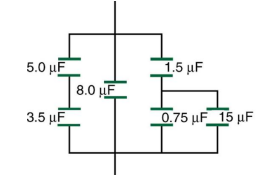
\includegraphics[scale=0.8]{cap}
		\end{center}
		\begin{enumerate}[label=(\roman*)]
			\item Find the effective capacitance of the network.\vspace{2.5in}
			\item If we applied a voltage of 6V between the top and bottom ends of the system, calculate the charge and energy stored in each capacitor.\vspace{3.5in}
		\end{enumerate}\newpage
		\subsection*{Chapter 3}
		\question Define current and explain current in different ways. For example, state why although capacitors can be treated as open switches, current still runs in the circuit.\vspace{1.5in}
		\question A conducting copper wire has a diameter of 2.228 mm. What magnitude current flows when the drift velocity is 1.00
		mm/s?\vspace{1.5in}
		\question Given that the density of Manganese is $3.7g/cm^3$ and that we assume that there are 3 mobile electrons per each atom, calculate the electron density of a conducting wire made of Manganese.\vspace{1.5in}
		\question Power outages are common in Ethiopia and hence rechargeable batteries are common. One such example of battery is a "power bank" that we can use to charge our devices. Aaron's "power bank" boasts a $6000mAh$ capability. What physical quantity does $mAh$ represent?\vspace{1.5in}
		\question Why are two conducting paths from a voltage source to an electrical device needed to operate the device?\vspace{1.5in}
		\question Why isn’t a bird sitting on a high-voltage power line electrocuted? What happens when it steps its feet on both wires?\vspace{1.5in}
		\question Discuss both the macroscopic and microscopic aspects of Ohm's Law.\vspace{1.5in}
		\question What is the effective resistance of a car’s starter motor when 200 A flows through it as the car battery applies 12.0 V to the motor?\vspace{1.5in}
		\question Find the conductivity and resistivity of a material if it is 50.0 m long with a 0.050 mm diameter and has a resistance of 80$\Omega$ at 20$^0$C?\vspace{2in}
		\question What does ammeter measure? How should it be connected to the circuit? Why? What about a voltmeter?\vspace{1.5in}
		\question If there are $n$ identical resistors of resistance R in a network and 40\% of them are connected in series while the other 60\% are connected in parallel, find the effective resistance in terms of n \& R. \vspace{1.5in}
		\question Given a battery, an assortment of resistors, and a variety of voltage and current measuring devices, describe how you
		would determine the internal resistance of the battery.\vspace{1.5in}
		\question The hot resistance of a flashlight bulb is $5\Omega$, and it is run by a 2.8-V alkaline cell having a internal
		resistance of $0.3\Omega$.
		\begin{enumerate}[label=(\roman*)]
			\item What current flows through the bulb?\vspace{1in}
			\item Calculate the power dissipated by the bulb.\vspace{1in}
			\item What is the efficiency of the battery?\vspace{1in}
		\end{enumerate} 
		\question Show that for two resistors $R_1$ and $R_2$, the effective resistance when they are combined is larger when the resistors are in series than when they are in parallel.\newpage
		\subsection*{Chapter 4}
		\question Discuss how the Hall effect could be used to obtain information on free charge density in a conductor.\vspace{1.5in}
		\question Explain why the magnetic field would not be unique (that is, not have a single value) at a point in space where magnetic field lines might cross. \vspace{1.5in}
		\question List the ways in which magnetic field lines and electric field lines are similar and different.\vspace{1.5in}
		\question The force per meter between the two wires of a jumper cable being used to start a stalled car is 0.225 N/m. 
		\begin{enumerate}[label=(\roman*)]
			\item What is the current in the wires, given they are separated by 2.00 cm?\vspace{1.5in}
			\item Is the force attractive or repulsive(\textit{the current carrying wires in a jumper cable run in opposite directions})?\vspace{1.5in}
		\end{enumerate}
		\question To what direction should an electron be shot so that when it is put in a magnetic field in the direction of the negative Z-axis, the force acting on it is in the positive X-axis?\vspace{1.5in}
		\question A cosmic ray electron moves at $ 7.50 \times 10^6 \;\textbf{m/s}$ perpendicular to the Earth’s magnetic field at an altitude where field strength is $1.00 \times 10^{-5} \;\textbf{T} $. What is the radius of the circular path the electron follows?\vspace{1.5in}
		\question Calculate the inductive time constant of a circuit which has an inductor with an inductance of 6mH and a resistor of resistance 300$\varOmega$. If the EMF supplied by the battery is 60V, calculate the time needed for the current to drop to 0.1A. \vspace{1.5in}
		\question Find the magnetic force(both the magnitude and direction) acting on a proton if its velocity is V=$1.6\times10^6\hat{\boldsymbol{j}}$ m/s and it is in a magnetic field of B=$2\hat{\boldsymbol{i}} + 8\hat{\boldsymbol{j}} + 72\hat{\boldsymbol{k}}$T\vspace{1.5in}
		\question Show that V/H and A/s are the same by doing a dimensional analysis.\vspace{1.5in}
		\question A long solenoid has 1000 turns uniformly distributed over a length of 0.40m. What current is required in the windings to produce a magnetic field of $\pi\times10^{-2}$G at the center of the solenoid?\vspace{1.5in}
		\question How can we decrease the effect of eddy currents?\vspace{1.5in}
		\question A 15.0 cm long rod moves at 6.00 m/s perpendicular to a magnetic field. What is the strength of the magnetic field if a 95.0 V emf is induced?\vspace{1.5in}
		\question Calculate the magnetic field strength needed on a 100-turn square loop 18.0 cm on a side to create a maximum torque of
		500Nm if the loop is carrying 25.0 A.\vspace{1.5in}
		\question What is the force and torque on a square-shaped 6A current carrying loop of conducting wire that has an area of 0.0064$m^2$ and surrounded by a permanent magnet with a field strength of B = $3.0\times10^5$T that is tilted at 30$^0$ to the loop?\vspace{1.5in}
		\question If a charged particle moves in a straight line through some region of space, can you say that the magnetic field in that region is necessarily zero?\vspace{1.5in}
		\question What is the angle between the current carrying wire and the magnetic field when the force exerted on the wire is half of the maximum force possible?\vspace{1.5in}
		\question Find the charge to mass ratio of a charge moving if it is moving at a speed of $v = 5.0\times10^3 m/s$ in a magnetic field of 0.08G and it has the same trajectory as an electron in the same magnetic field.\vspace{1.5in}
		\question What is the magnetic field 2cm away due to a straight current carrying wire made of Manganese if the wire has a volume $27cm^3$ and length 3cm, if it is switched on for 5 seconds?\vspace{1.5in}
		\question A uniform magnetic field of magnitude 1.2 T is directed along the negative y - axis. An electron moving at a speed of 0.2$c$ makes an angle of 60$^0$ with the y - axis. Answer the following questions.
		\begin{enumerate}[label=(\roman*)]
			\item What is the expected trajectory of the electron?\vspace{1.5in}
			\item Calculate the radius \& pitch of the trajectory.\vspace{1.5in}
		\end{enumerate}
		\question What are ferromagnetic materials? What are some common ferromagnetic materials?\vspace{1.5in}
		\question We have seen that charges and magnets have similar properties. How is a charge similar to and different from a magnet?\vspace{1.5in}
		\question If a current carrying wire of 2A and length 3m is in a region of space that is perpendicular to a magnetic field of 3T, what is the maximum force on the wire? What about the minimum force?\vspace{1.5in}
		\question An electron and a proton are shot with the same speed of $3\times10^7m/s$ perpendicular to the magnetic field in question 3. What are the magnitudes of the forces on the electron and the proton? What about the radius of the trajectories by the electron and the proton?\vspace{2in}
		\question A current carrying wire that is carrying a current of 4A is going into the page. What is the magnetic field strength due to the wire 2cm vertically above the wire?(Both B and $\hat{B}$)\vspace{1.5in}
		\question For two wires both going out of the page, show that the two wires attract.\vspace{1.5in}\newpage
		\subsection*{Chapter 5}
		\question Let's say we want to study a signal visually. For an AC signal of a maximum voltage 12V and frequency of 60 Hz, draw a visual representation of what we would expect to see on an oscilloscope. You are free to give the oscilloscope the time base and gain control of your choice.\vspace{1.5in}
		\question State the uses of a transistor and explain how amplification is possible through a double junction. Draw the paths of current in the transistor and state Kirchhoff's Law. Explain why the word "amplification" is misleading while using it for transistors.\vspace{1.5in}
		\question Explain the difference between P-type and N-type semiconductors and how they are made. Explain how their properties gives rise to rectification. Explain what rectification is and state what the opposite process of rectification is(inversion) and state how we can rectify or invert current.\vspace{1.5in}
		\question Define and explain the following terms:
		\begin{enumerate}[label=(\roman*)]
			\item  Doping and impurities.\vspace{1.5in}
			\item  Acceptor and Donor atoms.\vspace{1.5in}
			\item  Conduction band theory and lattice structures.\vspace{1.5in}
		\end{enumerate}
		\question Explain what we mean by 0 and 1 electrical signals. Explain what logic gates are. Give 3 examples of ligc gates used in real life.\vspace{1.5in}
		\question In what way can we achieve a full wave rectification?\vspace{1.5in}
		\question An input of direct current is sent into an unknown electrical device and when current emerges out of the device, the output current is alternating. What device could the unknown be?\vspace{1.5in}
		\question What is the emission of conduction electrons from the hot meta in a Fermi valve is known as?\vspace{1.5in}
		\question Why is the Fermi valve referred to as a "valve"?\vspace{1.5in}
		\question Check whether the logic gates given below are equivalent or not by preparing a table of truth values.
		\begin{choices}
			\choice An \textbf{AND} and a \textbf{NOT-NAND}\vspace{1in}
			\choice An \textbf{NOR} and a \textbf{NOT}\vspace{1in}
			\choice An \textbf{AND} and a \textbf{OR}\vspace{1in}
			\choice A \textbf{NOT} and an \textbf{XOR}\vspace{1in}
		\end{choices}
		\question What does it mean when a P-N junction is forward biased? What about when it is reverse biased?\vspace{1.5in}
		\question Why is rectification by a single diode always half-wave?\vspace{2.5in}
		\question Plot a signal for a CRO measuring a signal of frequency 200Hz and maximum voltage 8V if the gain control is 4V/cm and time base is 2ms/cm.\vspace{1.5in}
		\question The collector current of a transistor is 4.2 A for a base current of 3.4 mA. What is the current gain?\vspace{1.5in}
		\question The base current of a transistor is 5.4 A, and its current gain is 1200. What is the collector current?\vspace{1.5in}\newpage
		\subsection*{Chapter 6}
		\question What is the bouncing of waves when they encounter a different medium called?\vspace{1.5in} 
		\question Show that the speed of light in vacuum can be expressed in terms of the electric and magnetic constants in the following manner: $c=\dfrac{1}{\epsilon_0\mu_0}$.\vspace{1.5in}
		\question The period of a transverse electromagnetic wave is 1$\mu$s, what is its frequency? What about its wavelength?\vspace{1.5in}
		\question How is an electromagnetic field produced?\vspace{1.5in}
		\question Radar is used to determine distances to various objects by measuring the round-trip time for an echo from the object.
		\begin{enumerate}[label=(\roman*)]
			\item How far away is the planet Mars if the echo time is 1400 s?\vspace{1.5in}
			\item What is the echo time for a speeding car 100.0 m from a police radar unit?\vspace{1.5in}
		\end{enumerate}
		\question An object of height 10cm is placed in front of a convex mirror of radius 20 cm,  25 cm away from the mirror. Determine the height of the image, how far it is from the mirror, whether it is real or virtual and whether it is upright or inverted.\vspace{1.5in}
		\question If a mirror produces a real image that is four times as large as the object and the object is located 40cm from the mirror, what is the focal length of the mirror?\vspace{1.5in}
		\question What is the focal length of a makeup mirror that has a power of 1.50 D?\vspace{1in}
		\question If Apple comes up with an iPhone that has a camera whose zoom lens has an adjustable focal length ranging from 100.0 to 400 mm. What is its range of powers?\vspace{1in}
		\question A clear crystal is immersed in water, and you wish to identify it by finding its index of refraction. You arrange to have a beam of light enter it at an angle of 46$^0$, and you observe the angle of refraction to be 40$^0$. What is the index of refraction of the substance and its likely identity.\vspace{1.5in}	
	\end{questions}		
\end{document}